Let us now consider a $N$-body problem, with $N>2$ gravitationally interacting
objects. We will solve this system with the \textit{direct summation method}.
First, however, let us cast the problem in dimensionless units. The $N$-body
equation reads
\begin{align}
    \frac{d\vec{x}_i}{dt}
    &=\vec{v}_i \\
    m_i\frac{d\vec{v}_i}{dt}
    &=Gm_i\sum_{k\neq i}m_k\frac{\vec{x}_k-\vec{x}_i}{|\vec{x}_k-\vec{x}_i|^3}
\end{align}

\subsection{Show that with an appropriate scaling $\vec x=\xi\vec x'$,
    $\vec v=\Phi\vec v'$, $t=\tau t'$ and $m=\mu m'$ (with $\xi,\Phi,\tau$
    and $\mu$ constants) the equations for $N$-body dynamics can be brought 
    into dimensionless form, where the gravitational constant $G$ is absorbed
    into the variables. Which condistions must $\xi,\Phi,\tau$ and $\mu$ obey
    and how many of them can be freely chosen?
}
    \begin{itemize}
        \item chain rule $\Rightarrow\phi=\xi/\tau$
    \end{itemize}
    \begin{align}
        \frac{d\vec x_i'}{dt'}
        &=\vec v_i' \\
        m_i'\frac{d\vec v_i'}{dt'}
        &=m_i'\cdot\sum_{k\neq i}m_k'\cdot
        \frac{\vec x_k'-\vec x_i'}{|\vec x_k'-\vec x_i'|^3}
    \end{align}
    From now on we will do everything in dimensionless units.

\newpage
\subsection{Write an $N$-body code for arbitrary $N$ with the leapfrog 
    integration and a constant time step.
} 
    One way to prevent numerical divergences in case of very close encounters 
    is to use the \textit{softening length parameter} $\varepsilon$ and modify 
    the gravitational force among massive particles:
    \begin{equation}
        m_i\frac{d\vec v_i}{dt}
        =Gm_i\sum_{k\neq i}m_k\frac{\vec x_k-\vec x_i}
        {|\vec x_k-\vec x_i|^3 + \varepsilon^3}
    \end{equation}
    However, $\varepsilon$ should be small enough to keep the simulation 
    physically consistent. We set:
    \begin{equation}
        \varepsilon=LN^{-1/3}\cdot\frac{1}{10000},
    \end{equation}
    where $L$ is the typical size of the system in dimensionless units and 
    $N$ is the number of particles.

    \paragraph{As a simple test problem, solve the following sample binary 
        star problem: two stars of mass $1$ at initial locations 
        $\vec x_1=(-0.5,0,0)$, $\vec x_2=(+0.5,0,0)$ and initial velocities
        $\vec v_1=(0,-0.5,0)$, $\vec v_2=(0,+0.5,0)$. Choose an appropriate
        time step! Plot the resulting trajectories of both starts in the 
        $(x,y)$-plane (projection). Plot also the time evolution of the 
        relative error of the total energy of the system.
    } \ \\
        \\
        \begin{figure}[h!]
            \centering
            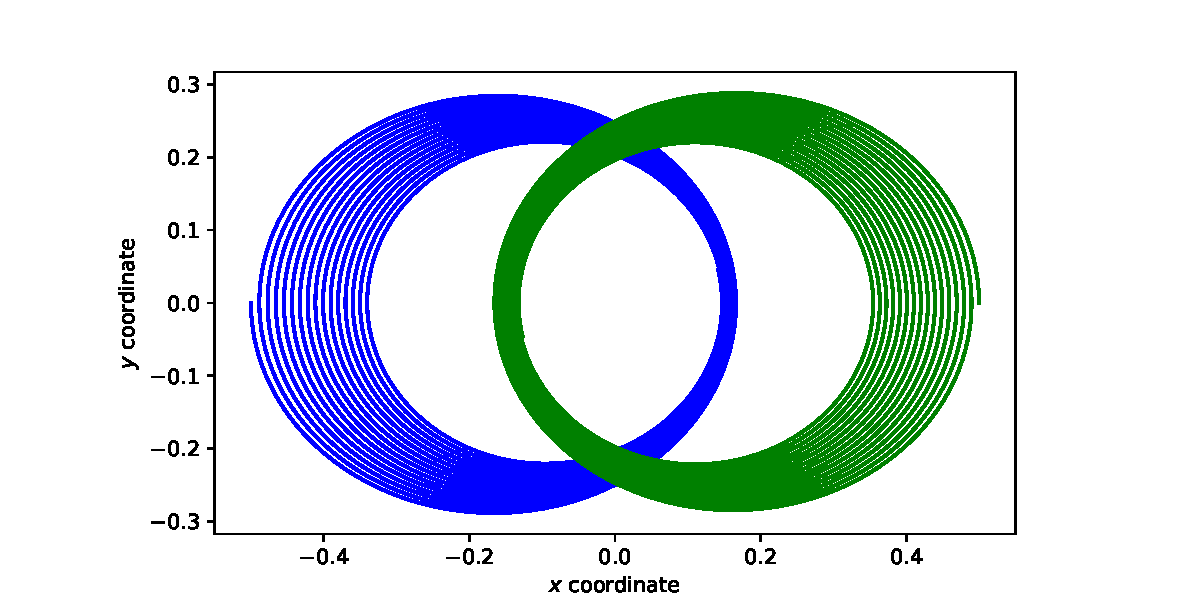
\includegraphics[width=\textwidth]{./figures/task2_2body.pdf}
            \caption{}
        \end{figure} \ \\ 

    \newpage
    \paragraph{Now add a third star with mass $0.1$ and initial position 
        $\vec x_3=(1,6,2)$ and initial velocity $\vec v_3=(0,0,0)$. Show how 
        this third star "falls into" the binary, interacts with it, and gets 
        eventually ejected. Plot the trajectories of all three stars in the 
        $(x,y)$-plane (projection). Again, plot the time evolution of the 
        relative error of the total energy of the system.
    } \ \\
        \\
        \begin{figure}[h!]
            \centering
            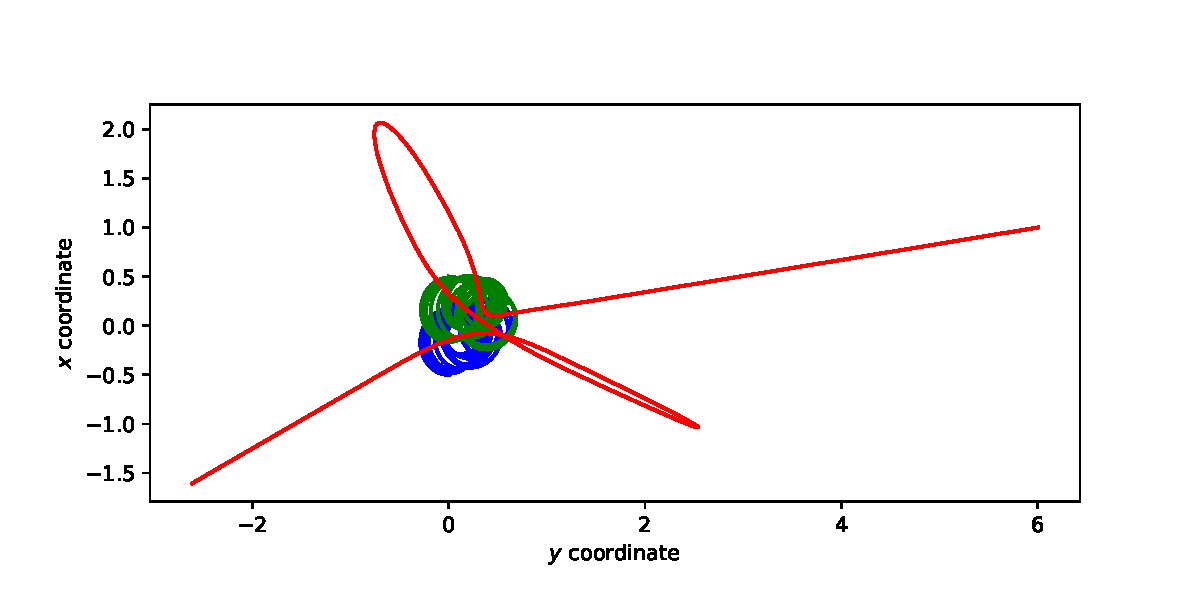
\includegraphics[width=\textwidth]{./figures/task2_3body.pdf}
            \caption{}
        \end{figure} \ \\ 
    
    \paragraph{Play with the time step by varying it at least a factor of 10 
        (but keep the final time of the integration fixed) and describe whether 
        the results change or not. The effect of changing the time step can 
        also be stronger than in this case, to see this also try 
        $\vec x_3=(1,6,3)$
    } \ \\
        \\
        \begin{enumerate}
            \item overall behavior is similar: star falls in, gets 
                "thrown around", then ejected
            \item details are different, e.g. direction of ejection
        \end{enumerate}

\newpage
\subsection{Real $N$-body problem ($N>>3$)}
    \paragraph{Set up a spherical cloud of 30 randomly positioned stars of 
        mass 1. The cloud radius is 1. Use a uniform random number generator 
        for this. An easy way is to choose randomly $(x,y,z)$ between 
        $-1$ and $+1$, and reject (and redo) stars that have 
        $1<\sqrt{x^2+y^2+z^2}$. Give each particle a random velocity
        (uniform) with a maximum of $0.1$. Use the same rejection trick as for 
        the positions. Evolve the system over an appropriate time-scale 
        (is there a characteristic time-scale for gravitationally interacting
        cluster?). 
    } \ \\
        \\
        For these simulations, we will have to use an adaptive time-step: at the 
        beginning of each iteration, we estimate the value of the time-step as 
        \begin{equation}
            \Delta t = C\cdot\frac{d_{min}}{|\vec v_{max}|},
        \end{equation}
        where $C=0.01\cdot d_{min}$ is the minimum distance between 2 particles 
        and $|\vec v_{max}|$ is the velocity of the fastest particle in the 
        system. If the evolution is unstable or if the relative error of the 
        total energy gets higher than 0.05, decrease the value of $C$ (note 
        that in this case you will need more iteration steps to evolve the 
        system to the same time scale).

    \paragraph{Plot the time evolution of the relative error of the total 
        energy.
    } \ \\
        \\ 
        ...

    \paragraph{Plot the evolution in 3D and note any interesting patterns that 
        emerge from the evolution. What are these? Why do they appear?
    } \ \\
        \\
        ...

    \paragraph{Now redo the simulation with $N=60$ and masses 0.5. Run this and 
        the previous simulation for 100 iterations each. Compare both the 
        results and run times between the two.
    } \ \\
        \\
        ...
